\cite{szegedy2014intriguing} was shortly followed up by \cite{goodfellow2015explaining}, which
brought to light strong evidence that the cause of these adversarial examples is the linearity of
the models being used (this linearity turns out to be limited, as discussed in \ref{tdlmrtaa}).
Mathematically, they point to the dot product that occurs in typical neurons and how drastically it
can change when only small changes to the input vector in the dot product occur. Analytically, they
come to this conclusion by pointing out that an adversarial example with noise $\eta$ for original
image $x$ will end up in the dot product with weight vector $w$ (note: all symbols used here are
from the paper); further, we added this equation for clarity, but keeping $w$ transposed instead of
the input vector):

$$w^T(x + \eta)$$

After distribution, they point out that the second term in the resulting addition is $w^T\eta$, a
non-negligible value (due to the number of elements participating in the dot product). They
end up drawing this conclusion: the dot product determines the final activation value, so, under a
max-norm constraint, noise added to a many-element vector may not appear to be much from the
max-norm perspective, but actually \textit{is} from the dot product perspective.

They bring up other theories about these phenomena, including the idea that nonlinearities are
causing them and that ``adversarial examples finely tile space like the rational numbers among the
reals''\cite{goodfellow2015explaining}[p. 7]. To debunk the first notion, they developed their own
attack called the \textit{Fast Gradient Sign Method} (FGSM). This attack consists of optimizing an
image by stepping away from the minimum, as opposed to towards it (the latter is the case in
training, and the parameters being optimized are that of the network instead of the image). This
uses the gradient (w.r.t. the image) of the actual loss of the image and its ground truth. However,
a modification here is that the sign of the gradient, after being multiplied by an
intensity-controlling value called $\epsilon$, is used in place of the gradient itself.

The goal of FGSM is two-fold. First, this method quickly generates adversarial examples instead of
normal iterative optimization found in \cite{szegedy2014intriguing}, as they point out. They state
that this makes training with adversarial examples (in addition to the regular images) much faster.
The second reason for its existence is to prove that the attack space is a continuously linear
subspace.

One reason that they note is simply because increasingly larger magnitudes of $\epsilon$ result in
even higher confidence in the same wrong class. However, the series of pictures in figure
\ref{imagegrid} that shows a visualization of the examples at those $\epsilon$ values shows the vast
majority of misclassified images being what they call ``rubbish examples'', and it appears that they
use that term to describe significantly fewer samples in that image than we would. There are only a
handful of misclassified subimages in that figure that, in our opinion, are actually recognizable
enough to not be considered rubbish.

\begin{figure}[th]
    \begin{center}
        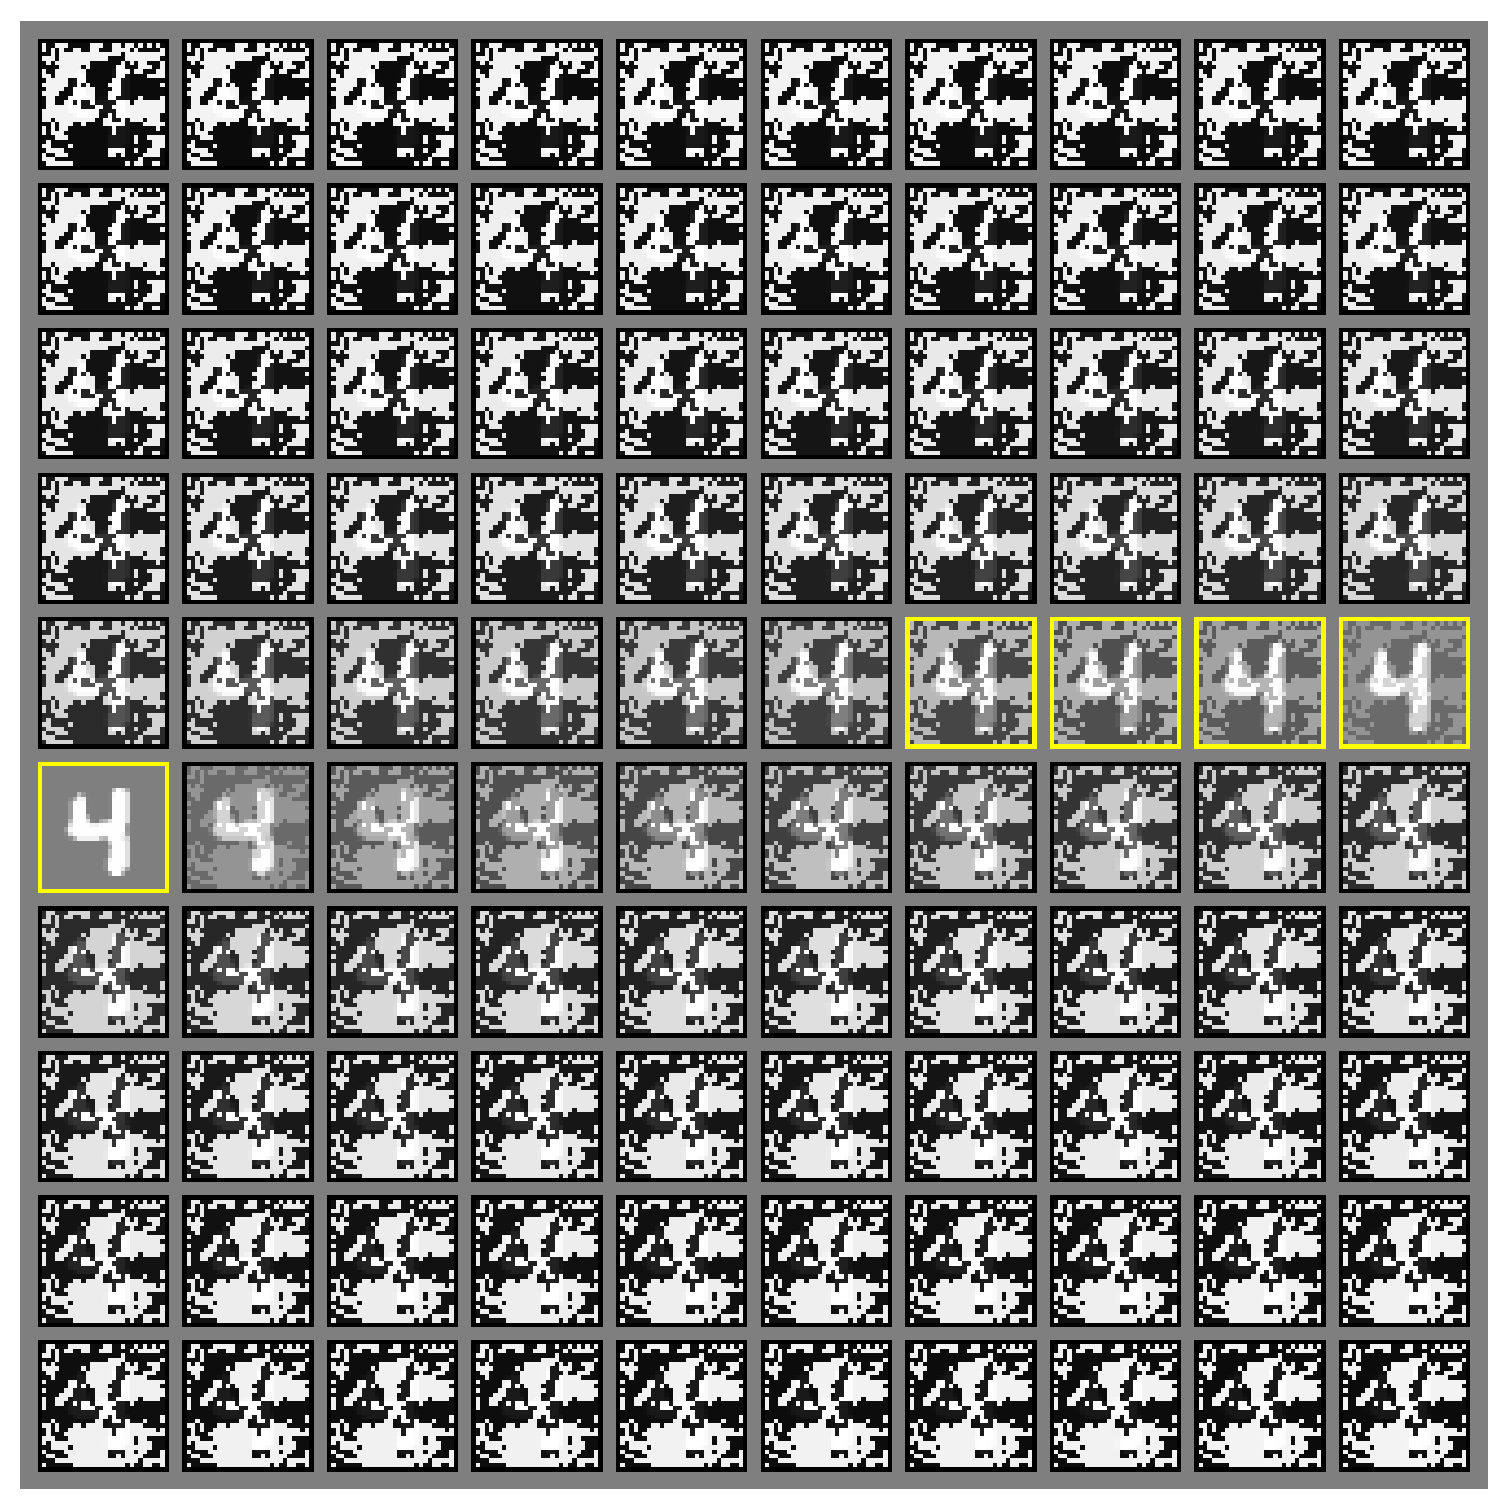
\includegraphics[width = 4in]{Friendly/LaTeX/figures/goodfellowdisagreement.png}
    \end{center}
    \caption{Part of figure 4 from \cite{goodfellow2015explaining}. The number of rubbish examples
             appears to be more than they indicate.}
    \label{imagegrid}
\end{figure}

A second thing that they point to is that adversarial examples created using a Radial Basis
Function-based network and a shallow neural network that uses Softmax (likely just on the logits of
the network) do not transfer as well to each other as the Softmax-based one does to a
Maxout~\cite{goodfellow2013maxout} network, which is more linear. A possibly important point to note
is that they state that the first network is ``shallow''\cite{goodfellow2015explaining}[p. 7], but
this author is not sure exactly what that means in the context of Maxout networks.